%%%% Proceedings format for most of ACM conferences (with the exceptions listed below) and all ICPS volumes.
\documentclass[sigconf]{acmart}
%%%% As of March 2017, [siggraph] is no longer used. Please use sigconf (above) for SIGGRAPH conferences.

%%%% Proceedings format for SIGPLAN conferences 
% \documentclass[sigplan, anonymous, review]{acmart}

%%%% Proceedings format for SIGCHI conferences
% \documentclass[sigchi, review]{acmart}

%%%% To use the SIGCHI extended abstract template, please visit
% https://www.overleaf.com/read/zzzfqvkmrfzn


\usepackage{booktabs} % For formal tables
\usepackage{graphicx}


% Copyright
%\setcopyright{none}
%\setcopyright{acmcopyright}
%\setcopyright{acmlicensed}
\setcopyright{rightsretained}
%\setcopyright{usgov}
%\setcopyright{usgovmixed}
%\setcopyright{cagov}
%\setcopyright{cagovmixed}


% DOI
%\acmDOI{10.475/123_4}

% ISBN
%\acmISBN{123-4567-24-567/08/06}

%Conference
%\acmConference[WOODSTOCK'97]{ACM Woodstock conference}{July 1997}{El
%  Paso, Texas USA} 
%\acmYear{1997}
%\copyrightyear{2016}


\acmArticle{4}
\acmPrice{15.00}

% These commands are optional
%\acmBooktitle{Transactions of the ACM Woodstock conference}


\begin{document}
\title{Face Recognition Based on Sparse Representation and Principal Component Analysis}
%\titlenote{Produces the permission block, and
%  copyright information}
% \subtitle{Extended Abstract}
% \subtitlenote{The full version of the author's guide is available as
%   \texttt{acmart.pdf} document}

\author{Qifan Zhang} 
\affiliation{%
 \institution{SIST, ShanghaiTech University}}
\email{47422183, zhangqf@shanghaitech.edu.cn}


% The default list of authors is too long for headers.


\begin{abstract}
This paper will achieve simple face recognition based on \emph{Principal Component Analysis (PCA)}. With the rising of training examples and proper parameters, accuracy could be up to 90\(\%\).
\\
The paper consists of 3 parts:
\begin{itemize}
	\item Introduction
	\item Algorithm Analysis
	\item Source Code Introduction
	\item Test and Results
	\item Problems and Possible Optimization
\end{itemize}
\end{abstract}

%
% The code below should be generated by the tool at
% http://dl.acm.org/ccs.cfm
% Please copy and paste the code instead of the example below. 
%


\keywords{Face Recognition, Principal Component Analysis, Sparse Representation}


\maketitle

\section{Introduction}

\emph{Face Recognition} is a very popular and common topic nowadays, especially in Computer Vision field. \emph{Face Recognition} involves many procedures, including generating and input of images, storage of face images, training of identification matrices, accuracy judgment and so on. 
\\
\emph{Sparse matrix representation} is a fast and storage-saving way to store and process signals, which makes it a more and more common method in signal processing. It focuses on what is useful and omit what is not, which is similar with the idea of \emph{eigenvalues (eigenfaces)}. Therefore, we use \emph{sparse representation classification} to do face recognition.

\section{Problem Formulation}
First, reduce dimension of dataset by PCA. Then find the projection with minimized error onto the new basis spanned by PCA. Then, test its accuracy.

\section{Algorithm Analysis}
I follow the procedure below to realize face recognition:
\begin{itemize}
	\item[1. ] Input training samples by placing each image column by column
	\item[2. ] Use \emph{Principal Component Analysis (PCA)} to omit redundant faces to reduce recognition time and collect eigenfaces
	\item[3. ] Implement SRBFR function, which is used to test accuracy of recognition. I use twenty images before recognition each person to get \(\lambda\).
	\item[4. ] Solve the \emph{minimum least-square error (MLSE)} to get sparse representations of test images
	\item[5. ] Judge unknown test images to face files by proportions in sparse representations of test images and see its accuracy
\end{itemize}

\subsection{Trainee Samples Input}

All of our images are \(192\times168\)\ .pgm images. We reshape each image into a column vector and attach them column by column to form a dataset matrix. Then train the data set by \(PCA\).

\subsection{PCA}
This is one of the most important steps in the whole procedure.
\\
\emph{PCA} is a theory that reduces dimension of a matrix to make it faster to compute and less space for it to store.
\\
I perform \emph{PCA} by:

\subsubsection{Calculate Covariance Matrix}
Definition for \emph{Covariance Matrix}:
\begin{displaymath}
	Cov = \frac{BB^{T}}{m-1}
\end{displaymath}
\(B\)\ is the \emph{the centred matrix} of dataset \(A\), which could be calculated by:
\begin{displaymath}
	B = A - ones(n,1)\times mean(A)
\end{displaymath}
Suppose \(A\)\ is a \(n\times m\)\ matrix, \(ones(n_A,1)\)\ generates a \(n\times1\)\ column vector with elements only 1. \(mean(A)\)\ is a \(1\times m\)\ row vector with mean of each column.

\subsubsection{Sigular Value Decomposition and Bases Change}
Theoretically, in order to get \(COEFF\), we should do \emph{Sigular Value Decomposition (SVD)} on \(Cov\). However, \(Cov\)\ is a \(32256\times32256\)\ matrix, which will consume a huge amount of time to do SVD.
\\
To optimize, we can calculate it in another way:
\[
	\begin{split}
		\frac{B^{T}B}{m-1}u &= \lambda u
		\\
		B\frac{B^{T}B}{m-1}u &= B\lambda u
		\\
		\frac{BB^{T}}{m-1}Bu &= \lambda Bu
		\\
		\frac{BB^{T}}{m-1}u' &= \lambda u'
	\end{split}
\]
\(u' = Bu\)
\\
Therefore, \(\frac{BB^{T}}{m-1}\)\ and \(Cov\)\ share the same eigenvalues while \(U' = BU\), \(U'\)\ is eigenvectors of \(Cov\)\ and \(U\)\ is eigenvectors of \(\frac{BB^{T}}{m-1}\).
\\
But the size of \(\frac{BB^{T}}{m-1}\)\ is \(m\times m\), which is largely smaller than \(Cov\)\ and much faster to get its SVD.
\\
To reduce \(A's\)\ dimension, we should only save eigenvectors that contribute more than 95\% to \(A\).
\\
In conclusion:
\[
	\begin{split}
		COEFF &= B \times U_k
		\\
		SCORE &= (COEFF)^{T} \times B
		\\
		LATENT &= \Sigma^{T}\Sigma \times ones(m,1)
	\end{split}
\]
\(U_k\)\ is a matrix containing first \(k\)\ eigenvectors that contributes more than 95\% to \(A\).

\subsection{SRBFR}
This is a program that tests accuracy using \(PCA\)\ with a given number of trainees.
\\
Firstly, I manually adjust \(\lambda\)\ in \emph{feature\_sign} in order to get the largest accuracy.
\\
I finally find out that when \(\lambda=0.0007\), the accuracy is the largest among every one.
\\
Then, we take out the last 20 figures in each file to test the accuracy of judgment, the result is in \textbf{Figure 1}.

\section{Data Description}
\subsection{PCA.m}
The function usage is:
\begin{displaymath}
	[COEFF, SCORE, LATENT] = PCA(X)
\end{displaymath}
Input:
\begin{itemize}
	\item[\textbf{A}:] a \(n\times m\)\ dataset matrix. Each column is a trainee image.
\end{itemize}
Output:
\begin{itemize}
	\item[\textbf{COEFF}:] a set of new basis, the size of \textbf{COEFF} is \(n\times k\)
	\item[\textbf{SCORE}:] the projection of the original data set \textbf{A} onto the new basis
	\item[\textbf{LATENT}:] a \(m\times1\)\ column vector containing eigenvectors of the covariance matrix of \textbf{A} in descendseing oreder.
\end{itemize}
\subsection{SRBFR.m}
The function usage is:
\begin{displaymath}
	[Accuracy] = SRBFR(numTrainee, path)
\end{displaymath}
Input:
\begin{itemize}
	\item[\textbf{numTrainee}:] the number of images in each candidate's file used to train the dataset.
	\item[\textbf{path}:] the \emph{filepath} to \emph{CroppedYale}
\end{itemize}
Output:
\begin{itemize}
	\item[\textbf{Accuracy:}] the average right-identification proportion of 20 test images from each file
\end{itemize}
\subsection{feature\_sign.m}
The function usage is:
\begin{displaymath}
	[x] = feature\_sign(A, y, lambda, [init\_x])
\end{displaymath}
\textbf{init\_x} is a zero vector by default.
\\
For a test image, we reshape it into a \(32256\times 1\)\ column vector \(y_0\).
\\
Then, we should project the test image onto the subspace of \textbf{COEFF} we got from PCA.
\\
So do \(B\).
\[
	\begin{split}
		A &= (B^{T}(COEEF)^{T})^{T}
		\\
		y &= (COEFF)^{T}y_{0}
	\end{split}
\]
\(\lambda\)\ is adjusted manually to achieve the largest accuracy.
\section{Test and Results}
I reserve 45 to 64 as test images while 1 to 44 are used for training and adjusting \(\lambda\). 
\\
All dataset are L2-normalized before calculated in \emph{feature\_sign}.
\\
The relationship between the number of trainees and accuracy is vividly shown in \textbf{Figure 1}.
\begin{figure}
	\centering
	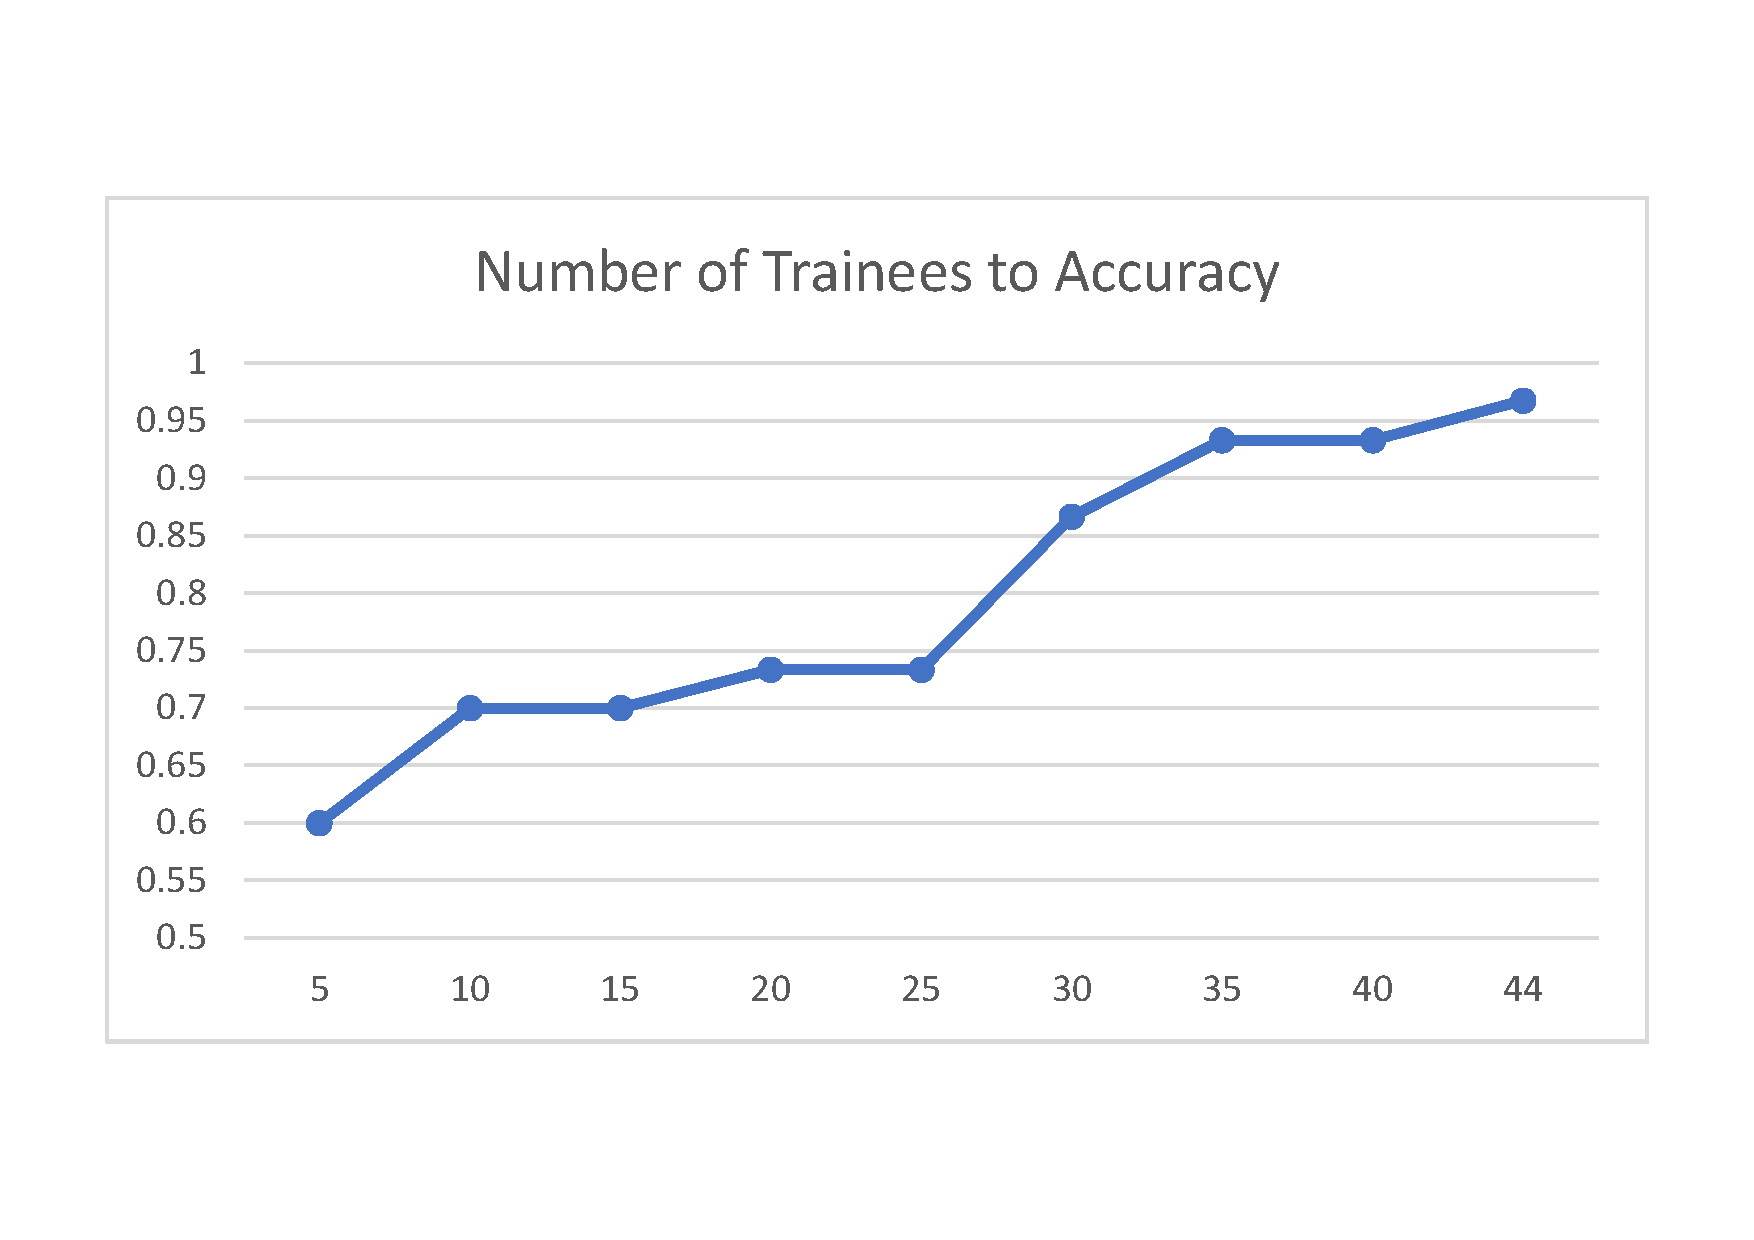
\includegraphics[width=0.7\columnwidth,height=0.6\linewidth]{Trainee_to_Accuracy.pdf}
	\caption{Trainee Number to Accuracy curve}
\end{figure}
Clearly, more dataset is used to train in PCA, more accurate the judgment is.
\\
The relationship between the number of trainees and time is vividly shown in \textbf{Figure 2}.
\begin{figure}
	\centering
	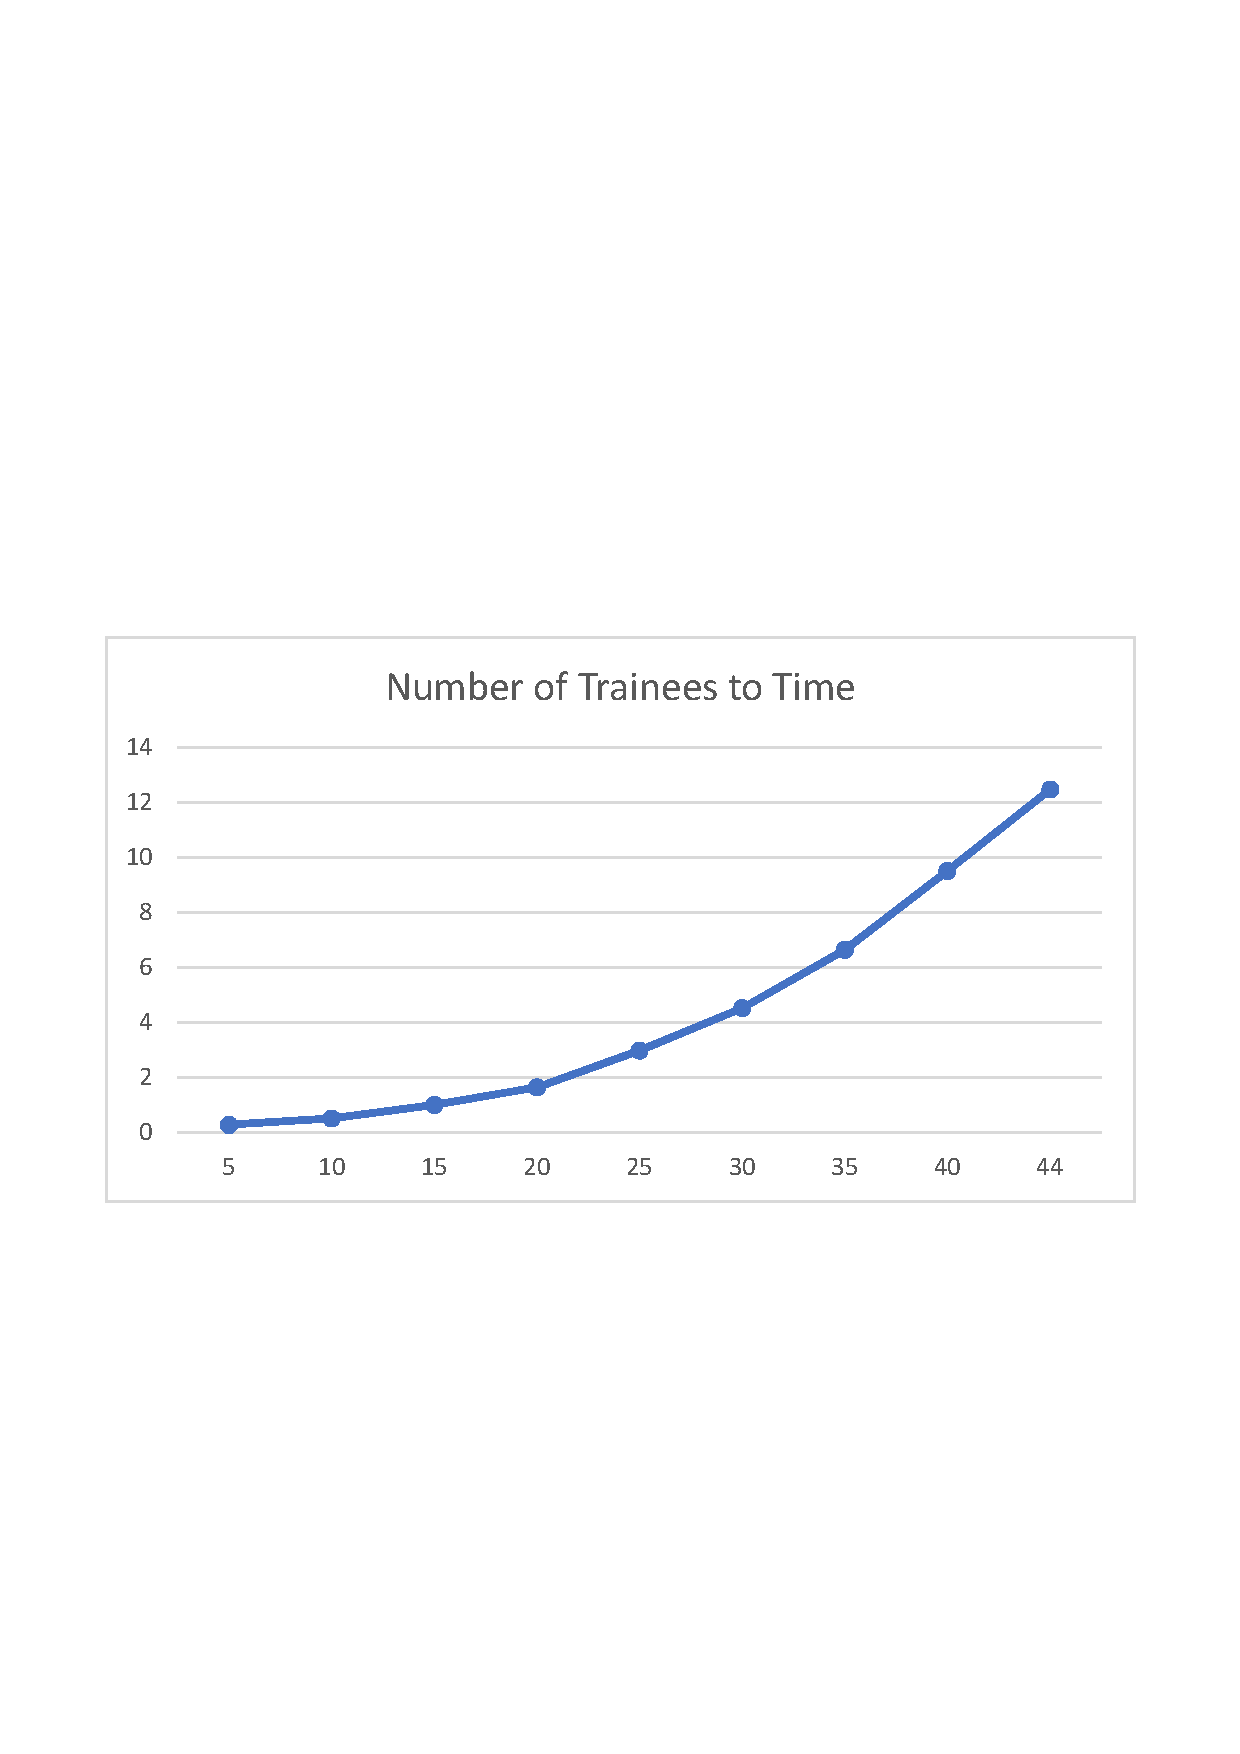
\includegraphics[width=0.7\columnwidth,height=0.9\linewidth]{Trainee_to_Time.pdf}
	\caption{Trainee Number to Accuracy curve}
\end{figure}
There is an almost exponential increase of time with the number of trainees.
\section{Observation and Possible Optimization}
\textbf{Figure 1} and \textbf{Figure 2} shows that times consumption has a positive relationship with the number of trainees. My PCA function is neither the best time-saving nor the best basis selection. If a better PCA procedure is required, \emph{Histogram Equalization} could be used according to documents I browsed online.
\\
Among all size of dataset, 30 may be the best size to train with not too much time consumption and a relatively high accuracy.
\\
I also find a fact that the ideal \(\lambda\)\ gets smaller with the increase of the serial number of test files. What is worse, the larger serial number of test file is, the lower accuracy \textbf{SRBFR} could achieve. In fact, I do not exactly know why. After discussion with my classmates, we think that maybe \textbf{SVD step changes the sequence of images we put in in order to get a descending order eigenvalues in \(S\).} But when we keep the sequence, the error gets smaller though, but a not large error is still there.
\\
Since these matrices are all matrices with double elements, GPU will do a much better job than CPU. If we could use GPU to compute, it will be bound to saving a lot of time.

\section*{Acknowledgment}
During this project, I discussed with \textbf{Huifan Zhang} and \textbf{Weitian Wang} about algorithm of PCA and SRBFR. I also refer to a lot of websites such as CSDN.com and Matlab Forum for support. The idea of optimization is inspired by papers in \emph{exampleWorks} on Piazza.com.

\section*{References}
\(\left [1 \right ]\): https://www.projectrhea.org/rhea/index.php/PCA\_Theory\_Examples
\\
\(\left [2 \right ]\): http://blog.csdn.net/watkinsong/article/details/8234766



\bibliographystyle{ACM-Reference-Format}
%\bibliography{sample-bibliography} 

\end{document}
